\scanpage{60}
% archive sheet number: 59

Par contre, si on fait un tour complet, de façon à revenir à l'orientation de départ de $D$, alors \deleted{\unsure{à}} (comme c'est le carré du lacet demi-tour) on trouve \deleted{que donc que on} \inserted{un transport parallèle} $\operatorname{Pol}(D)\longrightarrow\operatorname{Pol}(D)$ qui conserve l'orientation.

\deleted{Notons aussi que \deleted{le nb} pour le ``lacet-demi-tour autour de $s$'', \deleted{on ne} \inserted{quand} le nb de pas est pair, alors le résultat du transport parallèle sur les polygônes de \unsure{référence} donne, sur l'orientation le $=$ résultat que le transport parallèle ordinaire de l'orientation. Cel signifie que l'orientation change \deleted{\unsure{pour ce|pour}} le long de ce lacet, si $\nu(s)$ pair. Si $\nu(s)$ impair, alors le résultat via les $\operatorname{Pol}(D)$, et via transport ordinaire, n'est \deleted{pas} le $=$ --- \deleted{donc} comme l'orientation est \uline{conservée} par transport parallèle, elle ne l'est pas par transport ordinaire --- donc en tous cas, cette dernière change}

\deleted{Ceci vaut chaque fois qu'on a un circuit fermé sur $\mathcal X$ (circuit conçu comme des faces) tel que le transport par ordinaire change l'orientation de \deleted{\unsure{D|$\Delta$}} la position relative $D$. \deleted{Que le nb de opérations soit pair ou pas, pour} \inserted{Alors l'orientation de $\mathcal X$ change} le long sss le nb de pas élémentaires est pair. Balayer au dessus d'un pt compte comme 2, balayer au dessus d'une p.r. supersingulière compte comme 1.}

Voilà enfin une façon de voir que $\Pi_1(\deleted{\unsure{\widetilde{\phantom{X}}}}\mathcal X)\longrightarrow\mathbb D_{2n}$ est surjectif.

On peut \unsure{sur|d'} une p.r. \inserted{$D$} stable proche d'une p.r. supersingulière $D_0$,

\figure{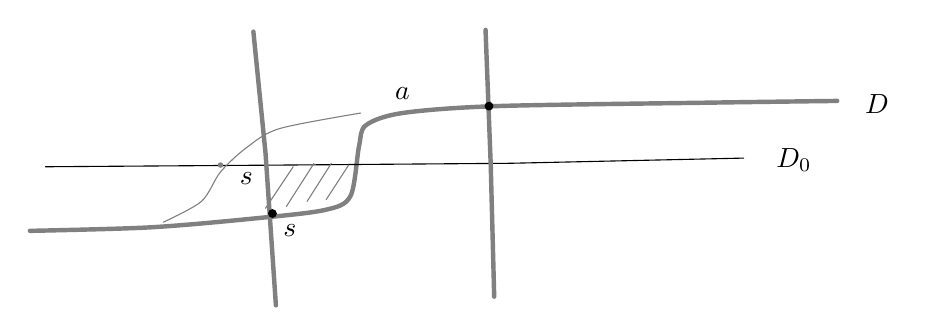
\begin{tikzpicture}[x=0.022cm,y=-0.022cm,line cap=round,line join=round]
\draw[gray,line width=1.6pt] plot[smooth] coordinates {(0,116) (69,114) (128,109) (170,104) (185,96) (190,67) (194,55) (215,48) (269,44) (392,42) (466,41)};
\draw[thin] (9,79)--(149,78)--(277,77)--(412,74);
\draw[gray,line width=1.6pt] (129,1)--(136,71)--(142,159);
\draw[gray,line width=1.6pt] (263,0)--(266,78)--(268,154);
\draw[gray,thin] plot[smooth] coordinates {(77,111) (99,99) (110,82) (125,68) (144,57) (191,48)};
\draw[gray,thin] (136,103)--(152,79);
\draw[gray,thin] (148,102)--(164,77);
\draw[gray,thin] (160,99)--(174,77);
\draw[gray,thin] (171,98)--(184,78);
\fill[black] (140,106) circle [radius=1.6pt];
\fill[black] (265,44) circle [radius=1.6pt];
\fill[gray] (110,78) circle [radius=1pt];
\node at (150,116) {$s$};
\node at (125,86) {$s$};
\node at (215,37) {$a$};
\node at (489,43) {$D$};
\node at (441,75) {$D_0$};
\end{tikzpicture}}
